% =========================================================================== %

\begin{frame}[t,plain]
\titlepage
\end{frame}

% =========================================================================== %

\begin{frame}[fragile]{Recap}
%
Letzte Stunde haben wir gesehen/kennengelernt:
%
\begin{columns}[T]
\column{.5\linewidth}
\begin{itemize}
\item die Arbeitsumgebung
	\begin{itemize}
	\item Code-Editor, Konsole
	\item Kompilieren, Programme Starten über die Konsole
	\item Script-Lösung \mintinline{text}{cr}
	\end{itemize}
\item die Grundlegende Struktur einer Code-Datei
	\begin{itemize}
	\item \mintinline{c}{#include}-Zeilen
	\item Hauptprogramm \mintinline{c}{int main () { ... }}
	\end{itemize}
\end{itemize}
%
\column{.5\linewidth}
\begin{itemize}
\item Variablen und Operatoren
	\begin{itemize}
	\item Datentypen (\zB \mintinline{c}{int}, \mintinline{c}{char}, \ldots)
	\item Hierarchie der Operatoren (\enquote{Punkt vor Strich})
	\end{itemize}
\item Befehl \mintinline{c}{printf} zur formattierten Ausgabe
\item \emph{Fragen hierzu?}
\end{itemize}
\end{columns}
%
\end{frame}

% =========================================================================== %

\begin{frame}{Recap}
%
\begin{columns}[T]
\column{.5\linewidth}
\begin{itemize}
\item die Zahlensysteme: Dezimal, Binär, Hexadezimal, Oktal
\item Pointer
	\begin{itemize}
	\item \enquote{Adresse} von Information im Speicher
	\item Nutzen: Meist Kommunikation mit anderen Programmteilen
	\end{itemize}
\item Dateneingabe mit \mintinline{c}{scanf}
\end{itemize}
%
\column{.5\linewidth}
\begin{itemize}
\item Bedingungsstrukturen
	\begin{itemize}
	\item \mintinline{c}{if-else}
	\item \mintinline{c}{switch-case}
	\item Schachtelung
	\end{itemize}
\item Logische Verknüpfung und Bitweise Logik
\item \emph{Fragen hierzu?}
\end{itemize}
\end{columns}
%
\end{frame}

% =========================================================================== %

\begin{frame}[fragile]{Aus den Übungen}
%
\begin{columns}[T]
\column{.6\linewidth}
\begin{codebox}
\begin{minted}[fontsize=\scriptsize,linenos]{c}
#include <stdio.h>
int main () {
  int   a = 21, b = 100;
  float c = 21, d = 100;
  
  printf("Ausgabe als Dezimalzahl:\n");
  printf("a: %d, b: %d\n"  , a, b);
  printf("c: %d, d: %d\n\n", c, d);
  
  printf("Ausgabe als Fliesskommazahl:\n");
  printf("a: %f, b: %f\n"  , a, b);
  printf("c: %f, d: %f\n\n", c, d);
}
\end{minted}
\end{codebox}
%
\column{.4\linewidth}
\begin{cmdbox}[Ausgabe]
\ttfamily\scriptsize
Ausgabe als Dezimalzahl:\newline
a: 21, b: 100\newline
c: 1, d: -2031822976\newline
\newline
Ausgabe als Fliesskommazahl:\newline
a: 0.000000, b: 0.000000\newline
c: 21.000000, d: 100.000000
\end{cmdbox}
%
\begin{hintbox}
Warnungen beachten!
\end{hintbox}
\end{columns}
%
\end{frame}

% =========================================================================== %

\begin{frame}[fragile]
%
\begin{cmdbox}[Compiler-Warnungen bei obigem Code]
\begin{minted}[fontsize=\scriptsize]{text}
myProgram.c: In function ‘main’:
myProgram.c:8:15: warning: format ‘%d’ expects argument of type ‘int’, but argument 2 has 
type ‘double’ [-Wformat=]
   printf("c: %d, d: %d\n\n", c, d);
              ~^
              %f
myProgram.c:8:22: warning: format ‘%d’ expects argument of type ‘int’, but argument 3 has 
type ‘double’ [-Wformat=]
   printf("c: %d, d: %d\n\n", c, d);
                     ~^
                     %f
myProgram.c:11:15: warning: format ‘%f’ expects argument of type ‘double’, but argument 2 
has type ‘int’ [-Wformat=]
   printf("a: %f, b: %f\n"  , a, b);
              ~^
              %d
myProgram.c:11:22: warning: format ‘%f’ expects argument of type ‘double’, but argument 3 
has type ‘int’ [-Wformat=]
   printf("a: %f, b: %f\n"  , a, b);
                     ~^
                     %d
\end{minted}
\end{cmdbox}
%
\end{frame}

% =========================================================================== %

\begin{frame}[fragile]{Aus den Übungen}
%
\begin{columns}[T]
\column{.6\linewidth}
\begin{codebox}
\begin{minted}[fontsize=\scriptsize,linenos]{c}
#include <stdio.h>
int main () {
  int   a = 21, b = 100, e;
  float c = 21, d = 100, f;
  
  printf("Fehler bei Division:\n");
    e = c/d;
    f = a/b;
  printf("e: %d\nf: %f\n\n", e, f);
	
  printf("Korrekte Division:\n");
    f = c / d;
  printf("f: %f\ndirekte Division: %f\n", 
    f, (float) a/b  );
}
\end{minted}
\end{codebox}
%
\column{.4\linewidth}
\begin{cmdbox}[Ausgabe]
\scriptsize
Fehler bei Division:\newline
e: 0\newline
f: 0.000000\newline
\newline
Korrekte Division:\newline
f: 0.210000\newline
direkte Division: 0.210000
\end{cmdbox}
%
\begin{hintbox}
Im Zweifel: Typecasting.
\end{hintbox}
\end{columns}
%
\end{frame}

% =========================================================================== %

\begin{frame}[fragile]{Aus den Übungen}
%
\begin{columns}[T]
\column{.5\linewidth}
\begin{codebox}[Gesehen]
\begin{minted}[fontsize=\scriptsize,linenos]{c}
...
disc = b*b - 4*a*c;
x1 = ( -b + sqrt(disc) ) / (2*a);
x2 = ( -b - sqrt(disc) ) / (2*a);

if        (disc > 0) {
  printf("Loesung 1: %lf\n", x1);
  printf("Loesung 2: %lf\n", x2);
} else if (disc = 0) {
  printf("Loesung: %lf\n"  , x1);
} else {
  printf("keine reellen Loesungen\n");
}
\end{minted}
\end{codebox}
%
\column{.5\linewidth}
\begin{codebox}[Empfohlen]
\begin{minted}[fontsize=\scriptsize,linenos]{c}
...
disc = b*b - 4*a*c;

if        (disc > 0) {
  printf("%lf, %lf\n", 
    ( -b + sqrt(disc) ) / (2*a), x2),
    ( -b - sqrt(disc) ) / (2*a), x2)
  );
} else if (disc = 0) {
  printf("%lf\n", -b / (2*a), x2));
} else {
  printf("keine reellen Loesungen\n");
}
\end{minted}
\end{codebox}
\end{columns}
%
\end{frame}

% =========================================================================== %

\begin{frame}[fragile]
%
\begin{columns}[T]
\column{.5\linewidth}
\begin{Large}
{Aus den Übungen}
\vspace{6pt}
\end{Large}
%
\begin{itemize}
\item \emph{Alle} möglichen Eingaben abfangen!
\item Weiteres Verhalten sonst kaum vorhersehbar
\item Absturz wahrscheinlich
\item Schwierig zu debuggen
\item Hier: \texttt{nan}: \emph{Not A Number}
\end{itemize}
\begin{warnbox}
Ich habe hieran schon viele Stunden verloren
\end{warnbox}
%
\column{.5\linewidth}
\begin{codebox}
\begin{minted}[fontsize=\scriptsize,linenos]{c}
#include <stdio.h>
#include <math.h>

int main () {
  float NotANumber; int x;
	
  NotANumber = sqrt(-1);  // -nan
  x = NotANumber;         // -2147483648
  printf("sqrt(-1) = %f\n", NotANumber);
  printf("x = %d\n", x);

  NotANumber = 1.0 / 0.0; //  inf
  x = NotANumber;         // -2147483648
  printf("1 / 0 = %f\n", NotANumber);
  printf("x = %d\n", x);
}
\end{minted}
\end{codebox}
\end{columns}
%
\end{frame}

% =========================================================================== %

\begin{frame}{Script}
%
\begin{itemize}
\item Kapitel 7
	\begin{itemize}
	\item 7.1. Programmsprünge: \mintinline{c}{goto}
	\item 7.2. Schleife mit Bedingung: \mintinline{c}{while}
	\item 7.3. Schleife mit Bedingung und einem garantierten Durchlauf: \mintinline{c}{do-while}
	\item 7.4. Zählschleifen: \mintinline{c}{for}
	\item 7.5. Eingriffe in den Kontrollfluss: \mintinline{c}{break und continue}
	\end{itemize}
\end{itemize}
%
\end{frame}

% =========================================================================== %

\begin{frame}[fragile]{Math-Library}
%
\begin{itemize}
\item Gängige Mathematische Problemstellungen schon gelöst. Z.\;B.: Wurzel einer Zahl
\item Header: \mintinline{c}{#include <math.h>}
\item Linken: Kommandozeilenoption \texttt{-lm}
\end{itemize}
%
\begin{cmdbox}[Kommandozeilenaufruf (minimal)]
gcc myCode.c -lm
\end{cmdbox}
\begin{cmdbox}[Kommandozeilenaufruf (empfohlen)]
gcc -std=c11 -Wall -Wextra -Wpedantic myCode.c -lm -o myExe
\end{cmdbox}
%
\end{frame}

% =========================================================================== %

\begin{frame}[fragile]{Mathematische Funktionen}
%
\begin{columns}[T]
\column{.5\linewidth}
\begin{itemize}
\item Nativ nur Grundrechenarten definiert
\item Bibliothek \texttt{libmath} definiert viele Lösungen
\item Im Code: \mintinline{c}{#include <math.h>}
\item Compileraufruf\newline 
	\texttt{gcc -lm [OPTIONS] [mycode.c]}\
\end{itemize}
Siehe auch\newline \url{http://www.cplusplus.com/reference/cmath/}
%
\column{.5\linewidth}
\begin{tcolorbox}[title=wichtige Funktionen]
\begin{table}
\footnotesize
\newcolumntype{C}{>{\ttfamily\centering\arraybackslash} p{.3\linewidth}}
\begin{tabularx}
	{\linewidth}
	{Cc}
	
	\normalfont Funktion & Wirkung \tabcrlf
	
	pow(a, b)   & Potenz: $a^b$ \\
	sqrt(x)     & Quadratwurzel: $\sqrt{x}$ \\
	exp(x)      & e-Funktion \\
	log(x)      & natürlicher Logarithmus \\
	sin(x)      & Sinus\\
	cos(x)      & Cosinus\\
	tan(x)      & Tangens\\
	asin(x)     & Arcussinus\\
	acos(x)     & Arcuscosinus\\
	atan(x)     & Arcustangens\\
	...
\end{tabularx}
\end{table}
\end{tcolorbox}
\end{columns}
%
\end{frame}

% =========================================================================== %

\begin{frame}[fragile]{Schleifen}
%
\begin{columns}
\column{.47\linewidth}
\begin{center}
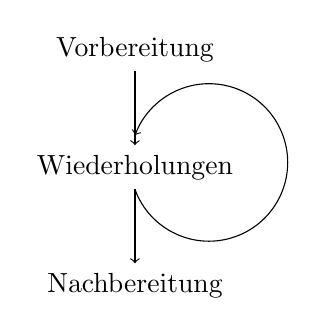
\begin{tikzpicture}
    \node at (0, 3  ) (Input)      {Vorbereitung};
    \node at (0, 1.5) (Operations) {Wiederholungen};
    \node at (0, 0  ) (Output)     {Nachbereitung};
    
    \draw [->] (Input) -- (Operations);
    \draw [->] (Operations.south)arc(-160:160:1.0);		%start angle: stop angle : radius
    \draw [->] (Operations) -- (Output);
\end{tikzpicture}
\end{center}
%
\column{.47\linewidth}
\begin{itemize}
\item Stärke von Computern: Wiederholungen
\item In schneller Folge gleichartige Arbeiten durchführen
\item Beispiel: Ähnliche Berechnungen
\item Kombinierbar mit anderen Blocks, wie z.\,B. \mintinline{c}{if}
\end{itemize}
\end{columns}
\end{frame}

% =========================================================================== %\\

\begin{frame}[fragile]{\mintinline{c}{goto} -- Sprunganweisung}
%
\begin{columns}[T]
\column{.47\linewidth}
\begin{itemize}
\item Setze Code-Ausführung an anderer Stelle fort
\item \enquote{Vorwärts-} und \enquote{Rückwärts-}Sprünge
\item Sprung zu \emph{Label}
\item Benennung wie Variablen
\item Spaghetti-Code -- nicht verwenden
\item Interne Umsetzung von \emph{Schleifen}
\end{itemize}
\begin{hintbox}
Sprechende Labels verwenden!
\end{hintbox}
%
\column{.53\linewidth}
\begin{codebox}[Beispiel: Wurzeln der Zahlen 1 bis 10]
\begin{minted}[fontsize=\scriptsize,linenos]{c}
#include <stdio.h>
#include <math.h>

int main () {
  double foo = 1;

  iterationPoint:
    printf("Wurzel aus %4.1lf: %lf.\n",
           foo, sqrt(foo));
    foo++;
  if (foo <= 10) {goto iterationPoint;}
    
  printf("Erfolgreicher Abschluss.\n");
}
\end{minted}
\end{codebox}
\end{columns}
%
\end{frame}

% =========================================================================== %

\begin{frame}[fragile]{\mintinline{c}{while}-Schleifen}
%
\begin{columns}[T]
\column{.4\linewidth}
\begin{codebox}[Syntax]
\begin{minted}[fontsize=\scriptsize,linenos]{c}
while (Bedingung) {
	Anweisungen
}
\end{minted}
%
\end{codebox}
\begin{itemize}
\item Wiederhole Anweisungen, während Bedingung erfüllt
\item Ausführung Zeile für Zeile
\item Prüfung am Anfang der Schleife
\item Komplettes Überspringen möglich
\end{itemize}
%
\column{.6\linewidth}
\begin{codebox}[Beispiel: Wurzeln der Zahlen 1 bis 10]
\begin{minted}[fontsize=\scriptsize,linenos]{c}
#include <stdio.h>
#include <math.h>

int main () {
  double foo = 1;

  while (foo <= 10) {
    printf("Wurzel aus %4.1lf: %lf.\n", 
           foo, sqrt(foo)
    );
    foo++;
  }
}
\end{minted}
\end{codebox}
\end{columns}
%
\end{frame}

% =========================================================================== %

\begin{frame}[fragile]{\mintinline{c}{do-while}-Schleifen}
%
\begin{itemize}
\item Variante der \enquote{normalen} \mintinline{c}{while}-Schleife
\item Einmalige Ausführung des Schleifeninhalts garantiert
\item Prüfung der Bedingung \emph{am Ende} statt \emph{am Anfang}
\end{itemize}
%
\begin{columns}[T]
\column{.5\linewidth}
\begin{codebox}[\mintinline{text}{do-while}]
\begin{minted}[fontsize=\scriptsize,linenos]{c}
#include <stdio.h>

int main(void) {
  int i = 10;
  
  do {
     printf("Schleifenkoerper\n");
  } while (i < 10);
  printf("Programmende\n");
}
\end{minted}
%
\end{codebox}
%
\column{.5\linewidth}
\begin{codebox}[\mintinline{text}{while}]
\begin{minted}[fontsize=\scriptsize,linenos]{c}
#include <stdio.h>

int main(void) {
  int i = 10;

  while (i < 10) {
    printf("Schleifenkoerper\n");
  }
  printf("Programmende\n");
}
\end{minted}
\end{codebox}
\end{columns}
%
\end{frame}

% =========================================================================== %

\begin{frame}[fragile]{\mintinline{c}{for}-Schleifen}
%
\begin{itemize}
\item \enquote{Zähl-Schleifen} -- für im Vornhinein bekannte Zahl von Durchläufen.
\item \enquote{Für jedes \texttt{i} zwischen \texttt{a} und \texttt{b} mache \ldots}
\end{itemize}
\vspace{-5pt}
%
\begin{columns}[T]
\column{.45\linewidth}
\begin{codebox}[Syntax]
\begin{minted}[fontsize=\scriptsize,linenos]{c}
for (Start; Bedingung; Iteration) {
   Anweisungen
}
\end{minted}
\end{codebox}
%
\begin{codebox}[Umsetzung]
\begin{minted}[fontsize=\scriptsize,linenos]{c}
Start;
while (Bedingung) {
   Anweisungen;
   Iteration;
}
\end{minted}
\end{codebox}
%
\column{.55\linewidth}
\begin{codebox}[Wurzeln der Zahlen 1 bis 10 \mintinline{text}{for}]
\begin{minted}[fontsize=\scriptsize,linenos]{c}
#include <stdio.h>
#include <math.h>

int main () {
  double foo;
  
  for (foo = 1; foo <= 10; foo++) {
    printf("Wurzel aus %4.1lf: %lf.\n", 
           foo, sqrt(foo)
    );
  }
}
\end{minted}
\end{codebox}
\end{columns}
%
\end{frame}

% ========================================================================== %

\begin{frame}[fragile]{Lebensdauer von Variablen: Scopes}
%
\begin{columns}[T]
\column{.45\linewidth}
\begin{itemize}
\item In \{Umgebungen\} können Variablen deklariert werden
\item Diese \enquote{existieren} nur \emph{innerhalb} der \{Umgebung\}
\item Betrifft: \mintinline{c}{if, switch, while, do, for, ...}
\item Bei \mintinline{c}{for}: Kurzform mit Gleichzeitiger Deklaraion und Initialisierung
\item Variable \enquote{lebt} nur innerhalb der Schleife
\end{itemize}
%
\column{.55\linewidth}
\begin{codebox}[\mintinline{text}{for} und Scopes]
\begin{minted}[fontsize=\scriptsize,linenos]{c}
#include <stdio.h>

int main () {
  for (int i = 1; i < 10; i++) {
    printf("%d\n", i);
  }
  
  // Fehler: i hier nicht mehr deklariert
  printf("%d\n", i);
}
\end{minted}
\end{codebox}
Mehr dazu später
\end{columns}
%
\end{frame}

% ========================================================================== %

\begin{frame}[fragile]{\mintinline{c}{break} and \mintinline{c}{continue}}
%
\begin{columns}[T]
\column{.5\linewidth}
\begin{tcolorbox}[title=\mintinline{text}{break}]
\begin{itemize}
\item Beendet Schleifen-Ausführung unabhängig von formaler Bedingung
\item Überspringt \emph{alle} folgenden Anweisungen
\item Code wird nach der aktuellen \{Umgebung\} fortgesetzt
\item Für zusätzliche Abbruch-Bedingungen
\item Vergleiche: \mintinline{c}{switch}
\end{itemize}
\end{tcolorbox}
%
\column{.5\linewidth}
\begin{tcolorbox}[title=\mintinline{text}{continue}]
\begin{itemize}
\item Springt zum nächsten Schleifen-Anfang
\item Schleife wird nicht verlassen/beendet
\item Bei \mintinline{c}{for}: Führt Iteration aus
\item Einzele Durchläufe überspringen, ohne Schleifenstruktur zu verwerfen
\end{itemize}
\end{tcolorbox}
\end{columns}
%
\end{frame}

% =========================================================================== %

\begin{frame}{Konsole -- Nützliche Tastenkürzel}
%
\begin{table}
\rowcolors{1}{white}{chameleonblue2}
\newcolumntype{A}{>{\ttfamily\arraybackslash} m{.35\linewidth}}
\newcolumntype{B}{>{\centering\arraybackslash} m{.6\linewidth}}
\begin{tabularx}
	{\linewidth}
	{AB}
	
	\normalfont Kürzel & Effekt \tabcrlf
	
	[CTRL] + [C] & Laufendes Programm sofort beenden \\
	
	[CTRL] + [SHIFT] + [C] & Markierten Text kopieren \\
	
	[CTRL] + [SHIFT] + [V] & Aus der Zwischenablage einfügen \\
	
	[Pfeiltaste nach oben] \newline
	[Pfeiltaste nach unten]   & 
	durch letzte Befehle scrollen \\
	
	[Tabulator] & Dateinamen vervollständigen \\
	
\end{tabularx}
\end{table}
Weitere Shortcuts: Siehe Link:
{\tiny \url{https://www.howtogeek.com/howto/ubuntu/keyboard-shortcuts-for-bash-command-shell-for-ubuntu-debian-suse-redhat-linux-etc/}}
%
\end{frame}

% =========================================================================== %

\begin{frame}[fragile]{Überblick: Schleifentypen}
%
Alle Schleifen für alle Zwecke \emph{geeignet} -- Empfehlung aber:
\begin{table}
\newcolumntype{S}{>{\ttfamily\centering\arraybackslash} m{.20\linewidth}}
\newcolumntype{U}{>{         \centering\arraybackslash} m{.30\linewidth}}
\newcolumntype{C}{>{         \centering\arraybackslash} m{.41\linewidth}}
\rowcolors{2}{cyan!25}{white}
\begin{tabularx}
	{\linewidth}
	{SUC}
	\toprule
	
	\normalfont \bfseries Schleife & 
	\bfseries Hauptzweck & 
	\bfseries Kommentare \tabcrlf
	
	for  &  Bekannte Zahl Durchläufe  &
	Schrittweite anpassbar \newline
	auch Variablen und Ausdrücke \newline 
	als Start/Zielwert/Iteration\\
	
	while  &  allgemeine Schleifen &
	Prüfung am Schleifenanfang\newline
	Überspringen möglich \\
	
	do-while  &  allgemeine Schleifen & 
	Prüfung am Schleifenende\newline
	ein Durchlauf garantiert\\
	
	\color{gray} goto & 
	\color{gray} selten sinnvoll &
	\color{gray} sprechende Labels verwenden! \\
	
	\bottomrule[1pt]
\end{tabularx}
\end{table}
%
\end{frame}

% =========================================================================== %

\begin{frame}{Script}
%
\begin{itemize}
\item Kapitel 6
	\begin{itemize}
	\item 6.1 Überblick über die Seite cppreference.com 
	\item 6.2 Funktionen zu einer Aufgabe finden 
	\item 6.3 Der Artikel zu sqrt
	\end{itemize}
\end{itemize}
%
\end{frame}

% =========================================================================== %

\begin{frame}{Nachschlagewerk: Die CPP-Referenz}
%
\begin{itemize}
\item Compiler erwartet exakten Umgang mit Syntax
\item Niemand erwartet, das alles nach zwei Wochen auswendig im Kopf zu behalten
\item Nachschlagewerk: \url{https://en.cppreference.com/w/c}
\item Gut sortierte Erklärung aller Standard-Befehle
\item C und C++
\item Hauptsprache Englisch; maschinell erstellte Übersetzungen verfügbar
\item Frei zugänglich, beständig aktualisiert
\end{itemize}
%
\end{frame}

% =========================================================================== %

\begin{frame}
%
\begin{columns}[T]
\column{.3\linewidth}
\begin{itemize}
\item Oben Links: Suchfeld
\item Unten: \enquote{In Other Languages}
\item Hauptteil: Sortierung nach Themengebieten
\item Grüne Markierungen: Features, die erst später hinzugefügt wurden
\item (Ähnliche Maske für C und C++ unter der Hauptseite \url{https://en.cppreference.com/})
\end{itemize}
%
\column{.7\linewidth}
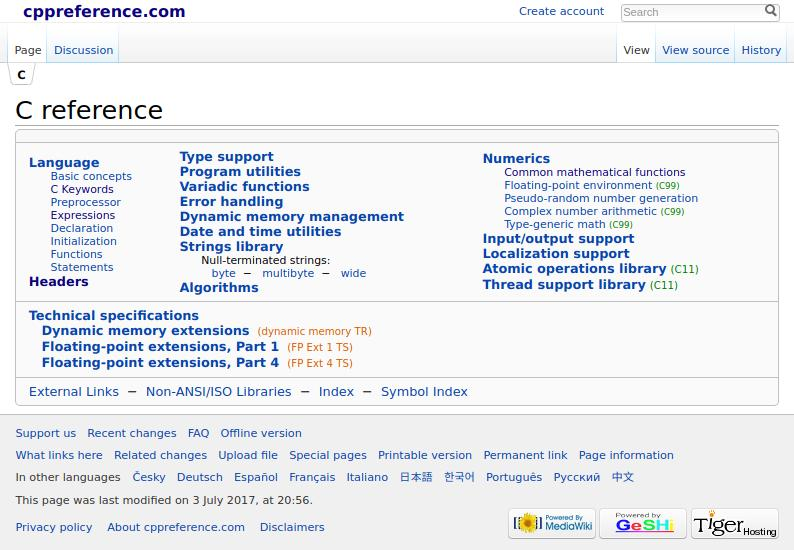
\includegraphics[width=\linewidth]{./gfx/cpp-home}
\end{columns}
%
\end{frame}

% =========================================================================== %

\begin{frame}
%
\begin{columns}%[T]
\column{.3\linewidth}
\begin{itemize}
\item Suchfunktion sowohl für C als auch C++
\item Einträge in Spalten sortiert
\item Ergebnisse: Auch ähnliche Schreibweisen
	\begin{itemize}
	\item Funktioniert also auch bei Tippfehlern oder unsicherer Schreibweise
	\end{itemize}		
\item Funktioniert in allen Spracheinstellungen
\end{itemize}
%
\column{.7\linewidth}
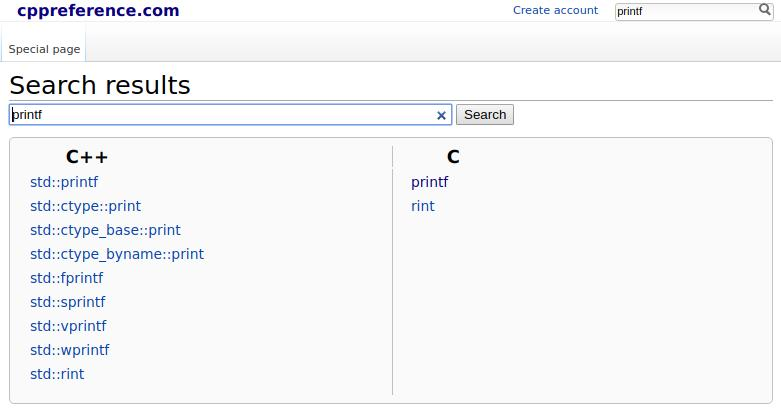
\includegraphics[width=\linewidth]{./gfx/cpp-search}
\end{columns}
%
\end{frame}

% =========================================================================== %

\begin{frame}
%
\begin{columns}%[T]
\column{.3\linewidth}
\begin{itemize}
\item Tatsächlich mehrere \enquote{verwandte} Befehle
	\begin{itemize}
	\item Schreiben auf Bildschirm, in Dateien, in sonstige Puffer
	\item Besonders gesicherte Versionen
	\end{itemize}
\item \emph{Prototypen}: Generische Liste aller Parameter und Rückgabetypen
\item Notwendiger \emph{Header} aufgelistet
\item Längerer Artikel, der alle Besonderheiten erklärt
\end{itemize}
%
\column{.7\linewidth}
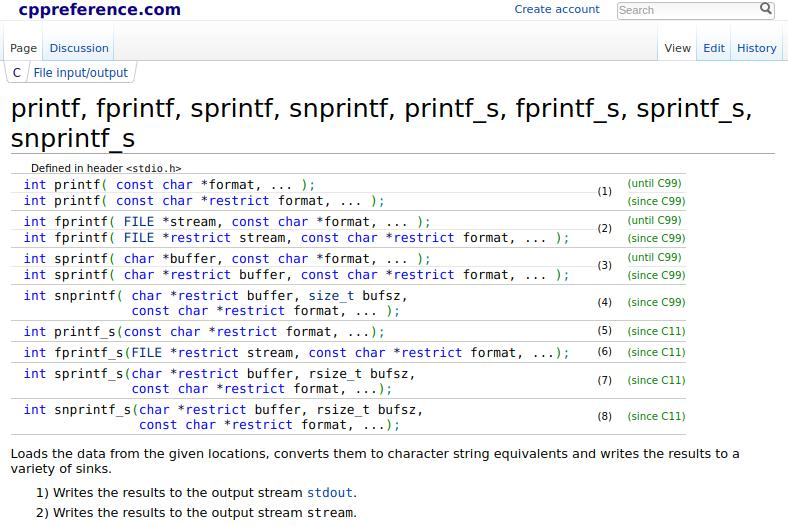
\includegraphics[width=\linewidth]{./gfx/cpp-printf}
\end{columns}
%
\end{frame}

% =========================================================================== %

\begin{frame}
%
\begin{columns}%[T]
\column{.3\linewidth}
\begin{itemize}
\item Suche nach Lösung zu bestimmter Aufgabe: Header durchsuchen
\item Gruppiert nach Aufgabengebieten
\item Liste von Header-Namen und Kurzbeschreibung der Lösungen darin
\end{itemize}
%
\column{.7\linewidth}
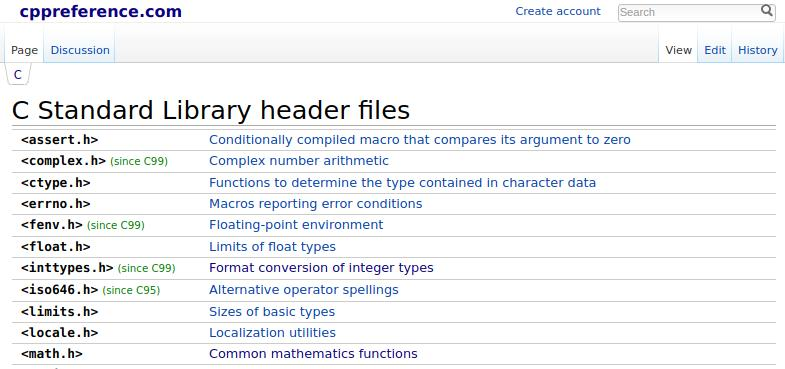
\includegraphics[width=\linewidth]{./gfx/cpp-headers}
\end{columns}
%
\end{frame}

% =========================================================================== %

\begin{frame}
%
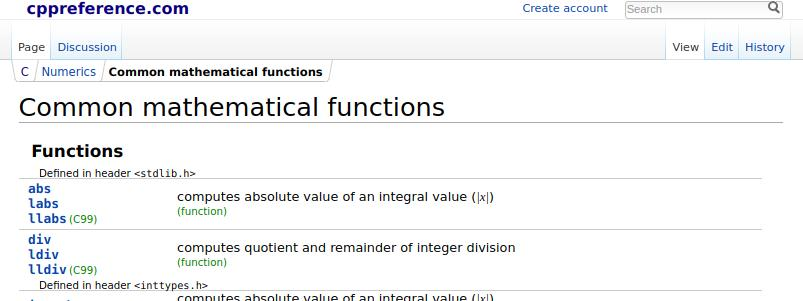
\includegraphics[width=\linewidth]{./gfx/cpp-math}
%
\begin{itemize}
\item Liste von Funktionen mit Kurzbeschreibung
\item Link zum Artikel
\item Benötigter Header und Compiler-Version bereits vermerkt
\end{itemize}
%
\end{frame}



% =========================================================================== %

\begin{frame}
%
\begin{columns}%[T]
\column{.3\linewidth}
\begin{itemize}
\item \texttt{sqrt}: Quadratwurzel einer Zahl berechnen
\item Unterschiedliche Varianten für verschiedene \emph{Datentypen}
\item Kurzbeschreibung
\item Erklärung der \emph{Parameter}
\item Erklärung des \emph{Rückgabewerts}, inclusive Verhalten bei Fehlern
\item Beispielcode
\end{itemize}
%
\column{.7\linewidth}
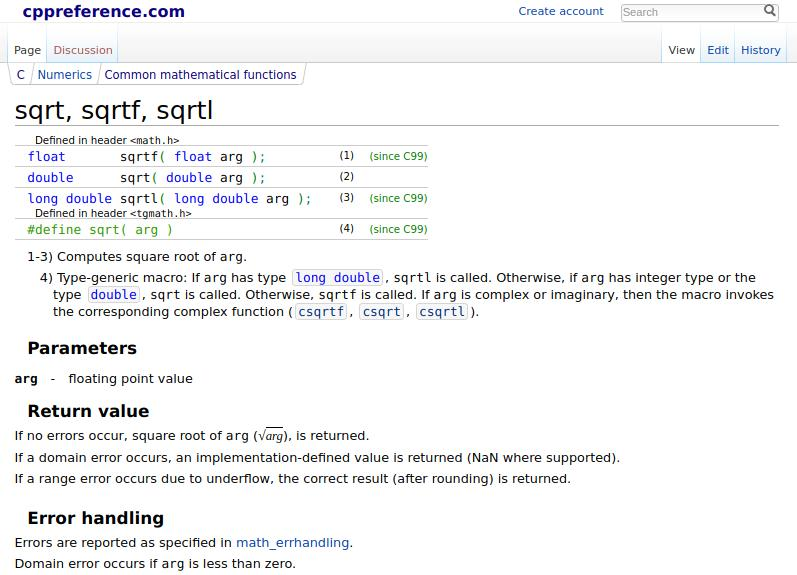
\includegraphics[width=\linewidth]{./gfx/cpp-sqrt}
\end{columns}
%
\end{frame}